\documentclass{beamer}

\usetheme{Boadilla}
\usecolortheme{beaver}

\usepackage{mathtools}
\usepackage{derivative}
\usepackage{amsthm}
\usepackage{tikz-cd}

\usepackage{graphicx}
\graphicspath{ {./images/} }

\DeclareMathOperator{\coker}{coker}
\DeclareMathOperator{\Hom}{Hom}
\DeclareMathOperator{\Coh}{Coh}
\DeclareMathOperator{\Crit}{Crit}
\DeclareMathOperator{\MF}{MF}

\newcommand{\A}{\mathbb{A}}
\newcommand{\C}{\mathbb{C}}
\newcommand{\Z}{\mathbb{Z}}
\renewcommand{\P}{\mathbb{P}}
\renewcommand{\O}{\mathcal{O}}
\newcommand{\calA}{\mathcal{A}}
\newcommand{\calB}{\mathcal{B}}
\newcommand{\calC}{\mathcal{C}}
\newcommand{\calD}{\mathcal{D}}
\newcommand{\calP}{\mathcal{P}}
\newcommand{\calE}{\mathcal{E}}
\newcommand{\calF}{\mathcal{F}}

\newcommand{\dL}{\mathbf{L}}
\newcommand{\dR}{\mathbf{R}}

\newcommand{\id}{\mathrm{id}}
\newcommand{\pt}{\mathrm{pt}}

\title{Derived categories of coherent sheaves}
\subtitle{(Introduction, and links to matrix factorizations)}
\date{15th May 2024}
\author{Calum Crossley}

\begin{document}

\begin{frame}
    \titlepage
\end{frame}

\begin{frame}
    \frametitle{Overview}

    \begin{itemize}
        \item Introduce derived categories of coherent sheaves

            (setting: smooth projective varieties over $\C$)

        \item Look at matrix factorizations

            (setting: affine hypersurface singularities)

        \item Two theorems: Kn\"orrer periodicity, cone singularities

            (relate matrix factorizations and derived categories)
    \end{itemize}
\end{frame}

\section{Derived categories of coherent sheaves}

\begin{frame}
    \frametitle{Coherent sheaves}

    Smooth projective variety $X/\C$. \pause

    ~

    Vector bundles (locally free sheaves): $\O^{\oplus 3}$, $\O(-1)$, $\ldots$
    \pause

    ~

    Coherent sheaves = (finite rank) vector bundles + cokernels

    $\to$ abelian category \pause

    ~

    Think vector bundles on subvarieties (sheaf pushforward), e.g. $\O_\pt$

    \begin{center}
        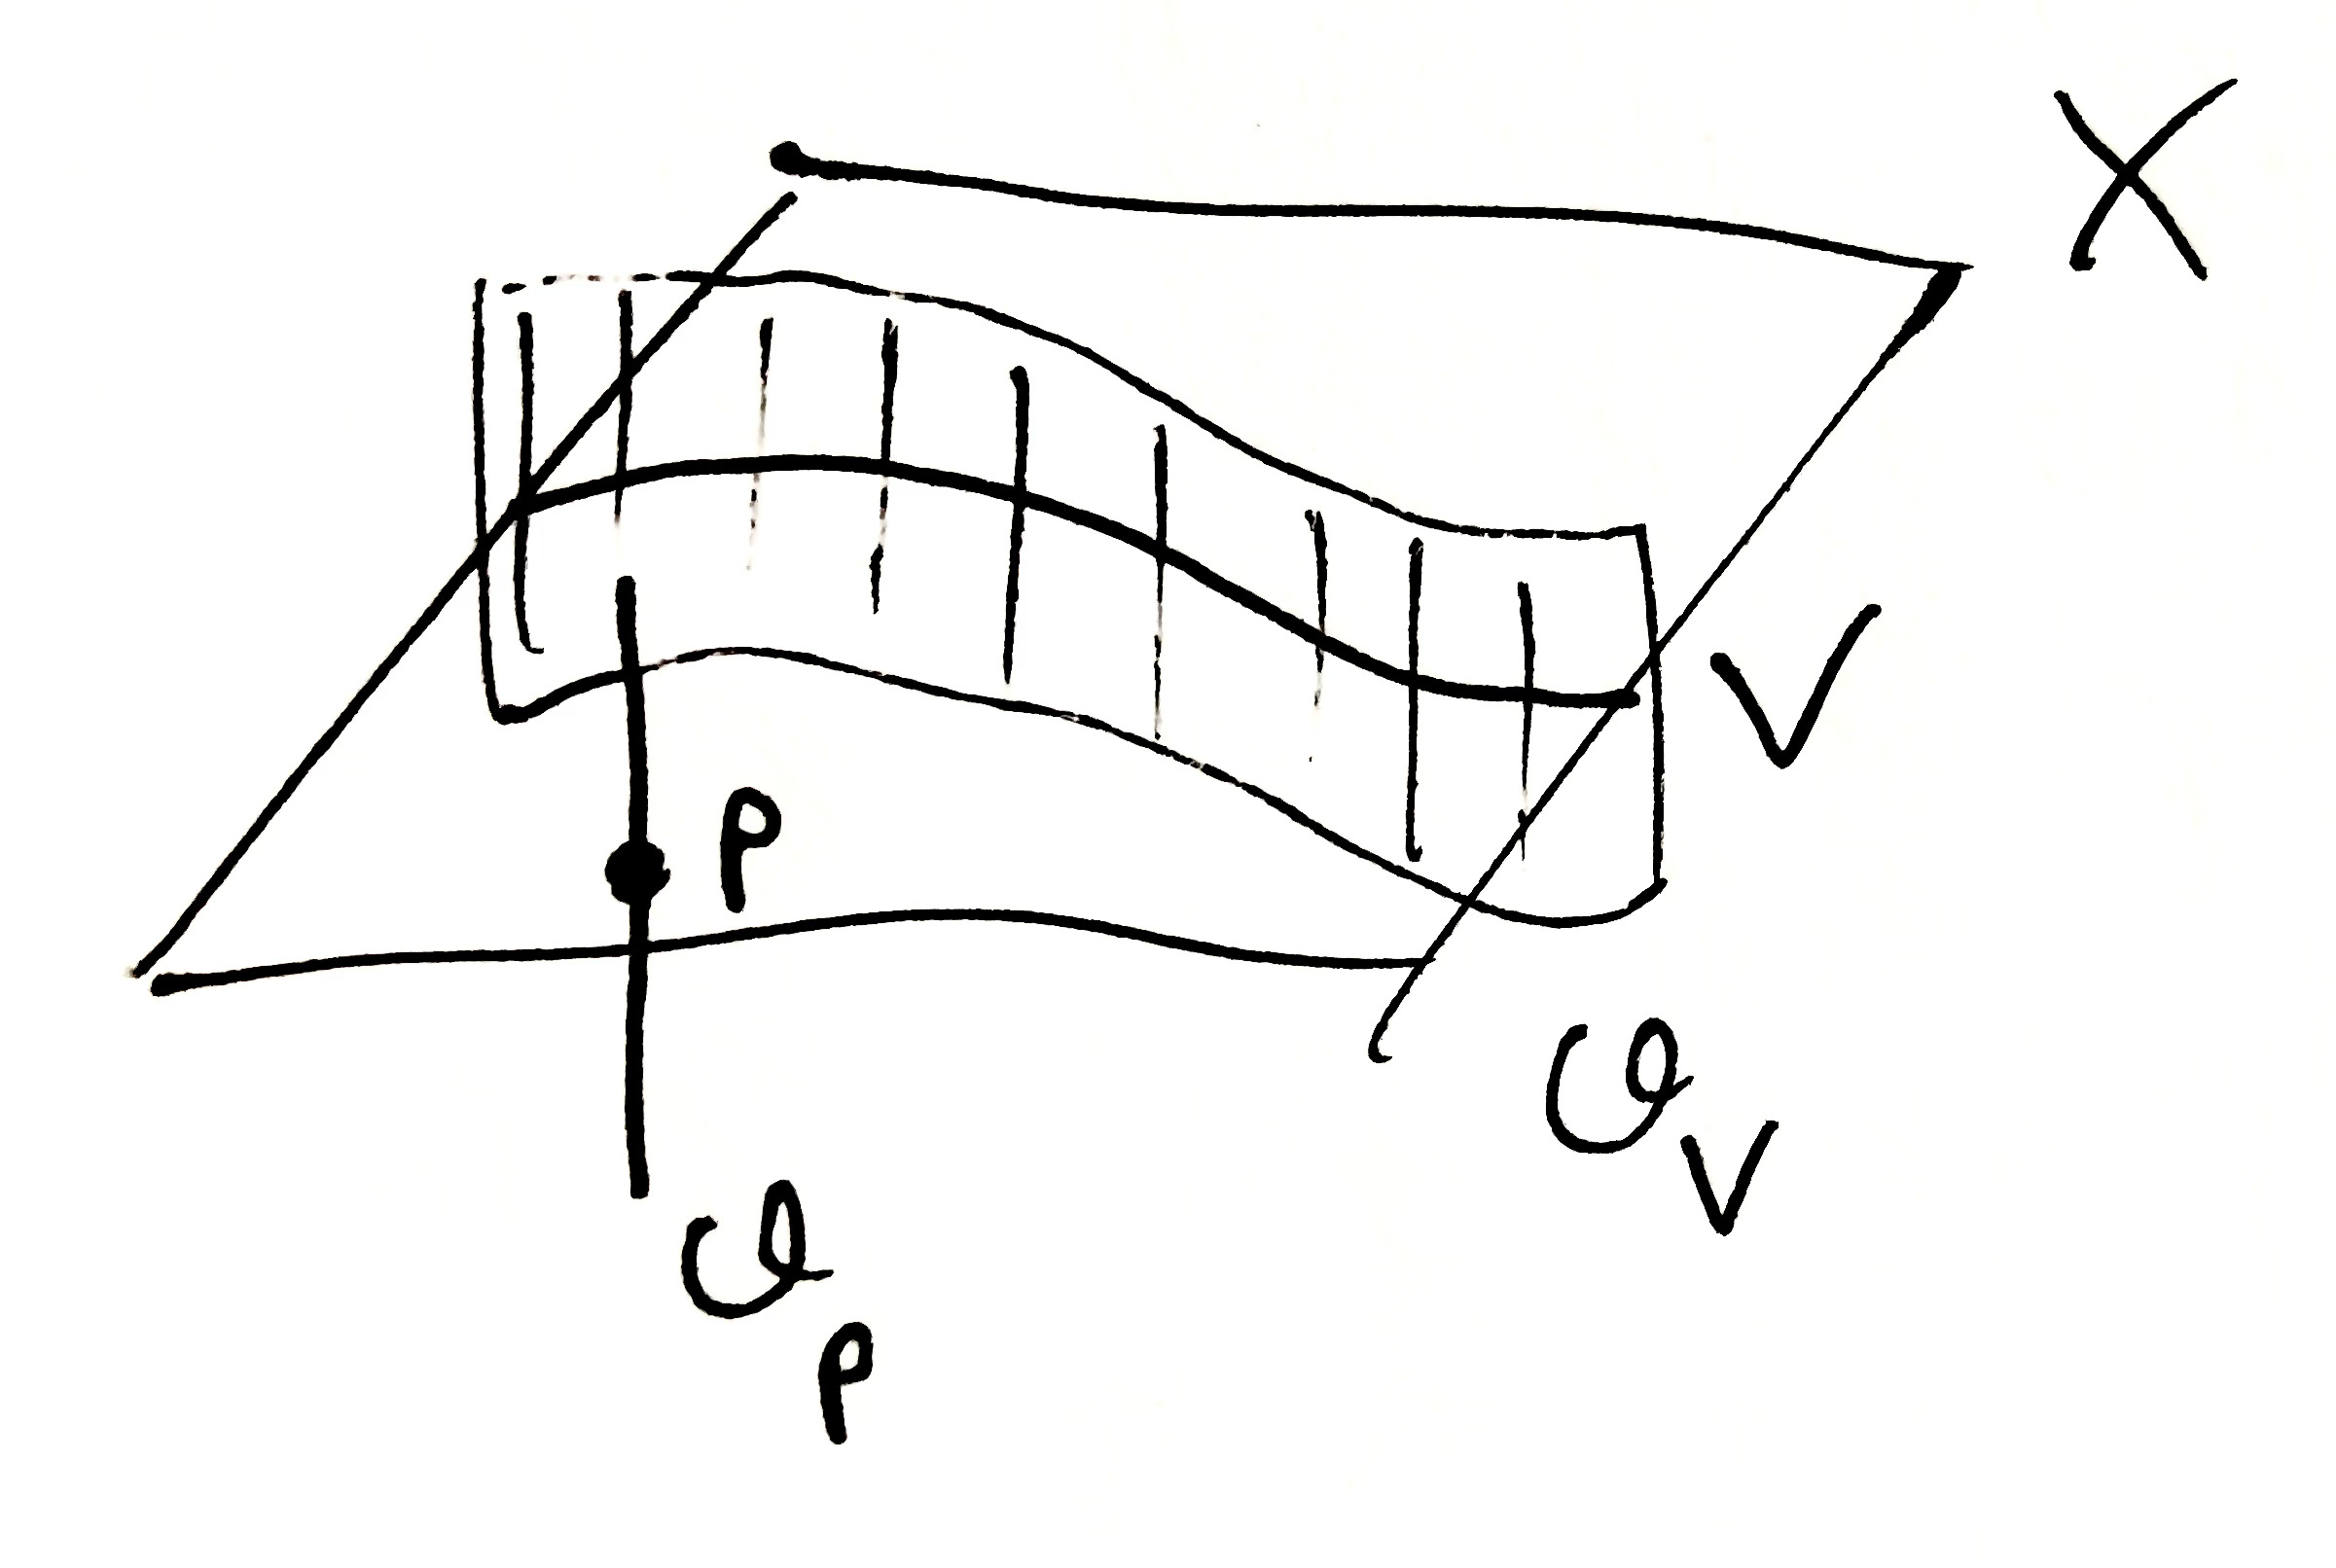
\includegraphics[scale=0.05]{coherent_sheaves}
    \end{center} \pause

    $\to$ $\Coh(X)$, determines $X$ (Gabriel-Rosenberg reconstruction)
    % technically that's QCoh, but Coh result also holds after Gabriel's results
    % Buan-Krause-Solberg, Support varieties -- an ideal approach, section 8
    % Garkusha-Prest, reconstructing projective schemes
\end{frame}

\begin{frame}
    \frametitle{Resolutions and derived functors}

    Sheaf cohomology: injective resolution, \v{C}ech resolution, LES

    ~

    Resolutions which are ``nice'' for global sections $\Gamma$, get more useful
    results \pause

    ~

    Tensor products = intersections

    Non-transverse? Use locally free resolutions ``nice'' for tensor products \pause

    ~

    $\O_H\otimes-$ applied to $\O_H$, replace by $\O(-H)\to\O$:
    $\O_H(-H)\xrightarrow{0}\O_H$

    ~

    Higher Tor detects self-intersection \pause

    ~

    Derived category = ``category of resolutions''

    Derived functor = ``functor applied to nice resolutions''
\end{frame}

\begin{frame}
    \frametitle{Technicalities}

    Resolution of $\calF$ = chain complex with cohomology $\calF[0]$

    ~

    Identify when quasi-isomorphic: $\exists$ comparison map identifying
    cohomology

    ~

    Restrict to bounded complexes, avoid infinite combinatorics $\to$
    $\calD(X)\coloneqq D^b(\Coh X)$. \pause \emph{Not} an abelian category \pause

    ~

    Left / right exact functor $F$ on $\Coh(X)$ $\to$ derived functor $\dL F$ /
    $\dR F$ on $\calD(X)$ via left / right ``nice'' ($F$-acyclic) resolutions if
    they exist

    ~

    Projective / injective resolutions are ``nice'', but no projective sheaves..

    Locally free ``nice'' for tensor products, $\Hom(-,\calF)$, pullback, $\ldots$

    ~

    Hilbert syzygy theorem: smooth projective $\implies$ bounded locally free
    resolutions
\end{frame}

\begin{frame}
    \frametitle{What can we do with them?} \pause

    Functor construction: Fourier-Mukai transforms: ``kernel''
    $\calP\in\calD(X\times Y)$ gives $\Phi_\calP:\calD(X)\to\calD(Y)$;
    $\calF\mapsto\dR(\pi_Y)_*(\calP\otimes^\dL(\dL\pi_X^*\calF))$

    ~

    { \color{gray}
    pushforward = $\dR\Gamma$ on fibers $\to$ ``integrate'' on fibers

    like integral transform
    $f(x)\mapsto\hat f(y)=\int_{X\times\{y\}}p(x,y)f(x)dx$
    } \pause

    ~

    Semi-orthogonal decompositions: split into objects / subcategories with
    (left/right) ``orthogonal complements'' wrt $\dR\Hom(-,-)$:

    ~

    $\calD(X)=\langle\calA,\calB,\calC\rangle$, no $\dR\Hom$'s right-to-left
    \pause

    ~

    e.g. Beilinson exceptional sequence:
    $\calD(\P^n)=\langle\O,\ldots,\O(n)\rangle$, SOD formulas for projective
    bundles, blowups, e.t.c.
\end{frame}

\begin{frame}
    $\calD(X)$ weaker than $\Coh(X)$, birational equivalences (e.g. flops) often
    give equivalences of $\calD(X)$ (D-K conjecture) \pause

    ~

    For Fano / anti-Fano does recover $X$ (Bondal-Orlov reconstruction) \pause

    ~

    Internal structure of $\calD(X)$ can be interesting, e.g. different SOD's,
    autoequivalences. See Bogdan's talk for example. \pause

    ~

    Kontsevich's homological mirror symmetry conjecture posits equivalence with
    symplectic geometry construction (Fukaya categories)
\end{frame}

\begin{frame}
    Now matrix factorizations:
\end{frame}

\section{Matrix factorizations}

\begin{frame}
    \frametitle{Resolutions with singularities}

    Cone $Z=\{xy=z^2\}\subset\A^3$. \pause
    Resolution for $L=\{x=z=0\}\subset Z$? \pause
    \begin{equation*}
        \cdots \to
        \O_Z^2 \xrightarrow{\begin{pmatrix}
            x & z \\ z & y
        \end{pmatrix}}
        \O_Z^2 \xrightarrow{\begin{pmatrix}
            y & -z \\ -z & x
        \end{pmatrix}}
        \O_Z^2 \xrightarrow{\begin{pmatrix}
            x & z
        \end{pmatrix}}
        \O_L\to0.
    \end{equation*} \pause
    ``Matrix factorization''
    \begin{equation*}
        \begin{pmatrix}
            y & -z \\ -z & x
        \end{pmatrix}
        \begin{pmatrix}
            x & z \\ z & y
        \end{pmatrix}
            = (xy-z^2)I =
        \begin{pmatrix}
            x & z \\ z & y
        \end{pmatrix}
        \begin{pmatrix}
            y & -z \\ -z & x
        \end{pmatrix}.
    \end{equation*} \pause

    Point: singular $\to$ infinite resolutions, often periodic ``matrix
    factorizations''
\end{frame}

\begin{frame}
    \frametitle{Matrix factorizations}

    Function $W$ on $\A^n$. \pause

    ~

    Make a category of matrix factorizations: \pause objects = vector bundles
    $(\calE^0,\calE^1)$ on $\A^n$ (i.e. trivial) with
    \begin{equation*}
        \begin{tikzcd}[ampersand replacement=\&]
            \calE^0 \ar[r,shift left,"d^0"] \&
            \calE^1 \ar[l,shift left,"d^1"]
        \end{tikzcd}
    \end{equation*}
    s.t. $d^1d^0=W\cdot\id_{\calE^0}$, $d^0d^1 = W\cdot\id_{\calE^1}$.
    ``$d^2=W$'' \pause

    ~

    $\Hom(\calE^\bullet,\calF^\bullet)$ gives $\Z/2$-graded total complex
    $\to$ differential $\Z/2$-graded category. \pause Take homotopy category:
    morphisms = $H^0$ of $\Hom(\calE^\bullet,\calF^\bullet)$ = chain maps up to
    chain homotopy \pause

    ~

    $\to$ $\MF(\A^n,W)$. \pause (graded vector bundles $\to$ $\MF_\Z(\A^n,W)$)
    % \Z/2-grading sad, want to recover \Z-graded chain complexes when W=0
    % d has grading 1, d^2 = W[2] (``W has grading 2'')
\end{frame}

\begin{frame}
    \frametitle{Relation to singularities}

    From $d^2=W$, have $d\pdv{}{x}(d)+\pdv{}{x}(d)d=\pdv{W}{x}$
    \pause $\leftarrow$ null-homotopy! \pause

    ~

    $\implies$ multiplication by derivatives of $W$ gives zero in $\MF(\A^n,W)$
    \pause

    ~

    $\implies$ matrix factorizations look like objects supported on
    $\Crit(\{W=0\})$. \pause

    ~

    Given $\calE^\bullet$, have sheaf $\coker d^0$ on $\{W=0\}$ with periodic
    resolution \pause
    \begin{equation*}
        \MF(\A^n,W) \simeq \calD(\{W=0\})
            / \{\text{finite locally free resolutions}\}
    \end{equation*}
    % sweeping technical details under rug
    % so matrix factorizations somehow account for all infinite resolutions
\end{frame}

\begin{frame}
    Now two theorems:
\end{frame}

\section{Kn\"orrer periodicity and cone singularities}

\begin{frame}
    \frametitle{Kn\"orrer periodicity}

    Suppose $MN=NM=W\cdot I$ is a matrix factorization. \pause

    ~

    Can factor $W+xy$:
    \begin{equation*}
        \begin{pmatrix}
            M & x \\ -y & N
        \end{pmatrix}\begin{pmatrix}
            N & -x \\ y & M
        \end{pmatrix}
            = (W+xy)I =
        \begin{pmatrix}
            N & -x \\ y & M
        \end{pmatrix}\begin{pmatrix}
            M & x \\ -y & N
        \end{pmatrix}.
    \end{equation*} \pause

    \begin{theorem}
        There is an equivalence $\MF(\A^n\times\A^2,W+xy)\simeq\MF(\A^n,W)$.
    \end{theorem}

    % example
    % line bundle generalization, critical locus

    % TODO
\end{frame}

\begin{frame}
    \frametitle{Cone singularities}

    Hypersurface $X=\{f=0\}\subset\P^n$, $f$ homog. degree $d$. \pause

    ~

    Affine cone $\{f=0\}\subset\A^{n+1}$ with $\MF_\Z(\A^{n+1},f)$ measuring
    singularity. \pause

    ~

    \begin{theorem}[Orlov]
        There is an equivalence $\MF_\Z(\A^{n+1},f)\simeq\calD(X)$.
    \end{theorem}

    % example
    % sketch via knorrer

    % TODO
\end{frame}

\end{document}
